\chapter{Background and literature search}

\iffalse
There are lots of different algorithms existing in the field of object detection and tracking. Some of those algorithms were investigated in this project in order to identify a set of suitable algorithms that were both accurate and efficient enough to analysis video stream from camera in real time.
\fi

Object tracking generally consists of 2 steps. Initially, locations and shapes of each moving object appeared in each frame need to be identified. Subsequently, by analysing and recording the movements of each object in sequential frames, the objects in a video stream can be tracked.

\section{Model based object detection algorithms}

\iffalse
Being able to detect objects in a video frame is the first, also the most important and challenging step to do object tracking. This is generally accomplished by separation of foreground objects and background image.
\fi

Object detection is generally accomplished by separation of foreground and background masks, called background subtraction or foreground segmentation.

\subsection{Colour based}
\label{bgs:colour}

Colour can sometimes provides enough information about a specific simple object, for example a coloured ball. For filtering a specific colour out from a video frame, hue-saturation-value (HSV) colour space \cite[p.~301]{colourspace} representation is usually used, which can makes colour filtering a lot easier based on hue, saturation and brightness information of the specific colour. In this way, a foreground mask can be generated easily by filtering target colour. For example, \fref{Figure:MOTBOC} shows a simple colour filtering object detection implementation \cite{MOTBOC.git} that is able to detect objects with specific colours.

\begin{figure}[H]
  \centering
  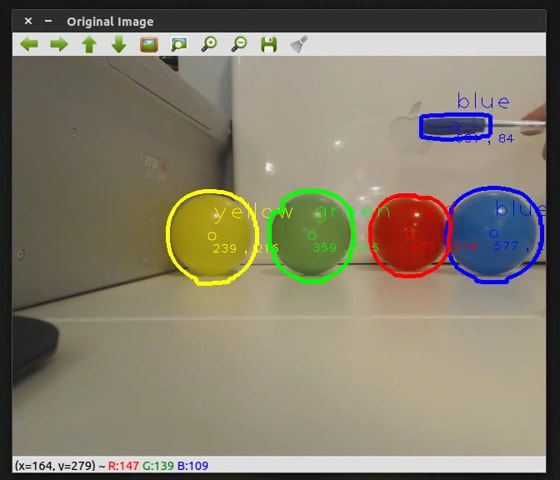
\includegraphics[width=0.6\columnwidth]{MOTBOC}
  \caption{Multi object tracking based on colour filtering (sourced from \cite{MOTBOC.git})}
  \label{Figure:MOTBOC}
\end{figure}

This implementation does not require a lot of graphic processing, thus can be made very quick and efficient, suitable for robots that are tracking something like a coloured ball or piece of paper, also could be useful for line racing car projects.

There are also researches using a more complex particle filtering algorithm based on colour distributions, such as \cite{nummiaro2003color}, results shown by \fref{Figure:nummiaro2003color}. {\color{red}Details on algorithm implementation required.}

\begin{figure}[H]
  \centering
  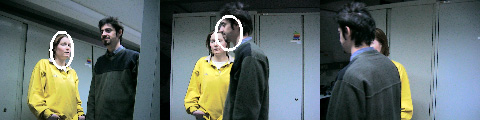
\includegraphics[width=0.9\columnwidth]{colour_based}
  \caption{Object detection based on colour distribution particle filtering (sourced from \cite{nummiaro2003color})}
  \label{Figure:nummiaro2003color}
\end{figure}

However, if there were other targets with similar colour, the algorithm may failed to distinguish them, as shown by the second image in \fref{Figure:nummiaro2003color}, {\color{red}Description...}. It also requires a specific model associated with each of the objects to be tracked.

\subsection{Shape based}

Another important information about an object might be its distinctive shape. By extracting object edges in the scene than apply appropriate shape transformation and filtering algorithms, an object could be detected based on its shape.

{\color{red}Use this research: \cite{borovicka2003circle}, and images?}

This implementation could be suitable for ball tracking purpose. By combining with the simple colour filtering algorithm as described in Section \ref{bgs:colour}, a single coloured ball could be efficiently tracked.

\subsection{Feature detection (Cascaded classifier)}

{\color{red}Use this: \cite{viola2001rapid}}

Cascade classifier \cite{cascade} is another widely used technique. It concatenates several classifiers detecting different object features to finally recognise objects, and its accuracy can be improved by training the classifier both positively and negatively. It was usually used not only for object detection, but also for object classification, for example recognise human and different classes of vehicles in a single frame.

{\color{red}Replace with results from research paper}

\section{Motion based object detection algorithms}

\subsection{Background subtraction}
\label{motion_bs}

By differencing current frame and previous frames then probably build up a background model image, it is also possible to detect moving objects efficiently.

{\color{red}Add some graph from research paper?}

{\color{red}Should be in design section?

This type of algorithms suit well for static camera movement tracking, and were not limited by objects' geometry shapes, therefore was used in this project.}

{\color{cyan}Background subtraction algorithms:

The BGS library

The BGSLibrary \cite{bgslibrary} is specifically developed for this purpose, it offers 37 different background subtraction algorithms implemented using OpenCV, published under GNU GPL v3 license.

Patented ViBE algorithm}

\subsection{Optical flow}

{\color{cyan}
Sparse feature set.
Dense optical flow.
}

\section{Object tracking algorithms}
\label{bg:tracking}

\subsection{Connected component analysis}
\label{blob}

After obtained the foreground object mask by some of the methods described above, it need to be interpreted as distinct objects, so that the geometry properties of each object can then be retrieved.

Connected component analysis, or Connected component labelling, is used for detecting connected regions (blobs) with the same colour, which are the possible regions of individual objects if applied to the foreground masks, therefore parameters such as shape, size and location of the objects can then be obtained.

There were also lots of free and open source blob detection libraries available, e.g. the simple blob detector came with OpenCV \cite{opencv:blob}, cvBlob library \cite{cvblob}.

After determined bounding shape, or region of interest (ROI) of an object by methods described before, the object can then be tracked between adjacent frames by labelling the blobs. Movement parameter such as velocity and acceleration may also be obtained by using physical modelling.

\subsection{Meanshift \& CAMshift}

Meanshift \cite{fukunaga2013introduction} is an algorithm used to track the movement of a fixed size ROI window between adjacent frames, by finding the peak of probability distribution of the ROI from the new frame. {\color{red}It can be easily implemented with OpenCV \cite{opencv:camshift}.}

{\color{red}Examples?}

\subsection{Continuously Adaptive Meanshift}

Continuously Adaptive Meanshift (CAMshift) \cite{bradski1998computer} is an algorithm based on Meanshift algorithm, that can handle target object size changing and rotation by iterating over the ROI to find the most suitable configuration. This algorithm can also be easily implemented using OpenCV \cite{opencv:camshift}, and was used by lots of researches for tracking purpose, such as \cite{chu2007object}, \cite{xu2012moving} and \cite{nouar2006improved}.

{\color{red}Examples?}

\subsection {Optical flow}

By evaluating pixel movements of feature points around ROI, the speed of a moving object relative to camera sensor space can be determined.

{\color{red}More..!}

\section{Object recognition}

Object recognition can also be developed by applying different cascade classifiers to the ROI of the specific object. This process is very computation intensive and time consuming, therefore should be executed as few as possible to achieve maximum power saving, for example, only execute once when the object first enter the sense or at its maximum visible size to the camera.

\section{Automatic feedback control}

Research about energy-efficient object detection by utilising hardware-level operations exists \cite{casares2011energy}, achieved an energy consumption reduction by $54.136\%$. But it was done on a very different and limited platform, also possible to extend further.
